\documentclass{article}\usepackage[]{graphicx}\usepackage[]{color}
%% maxwidth is the original width if it is less than linewidth
%% otherwise use linewidth (to make sure the graphics do not exceed the margin)
\makeatletter
\def\maxwidth{ %
  \ifdim\Gin@nat@width>\linewidth
    \linewidth
  \else
    \Gin@nat@width
  \fi
}
\makeatother

\definecolor{fgcolor}{rgb}{0.345, 0.345, 0.345}
\newcommand{\hlnum}[1]{\textcolor[rgb]{0.686,0.059,0.569}{#1}}%
\newcommand{\hlstr}[1]{\textcolor[rgb]{0.192,0.494,0.8}{#1}}%
\newcommand{\hlcom}[1]{\textcolor[rgb]{0.678,0.584,0.686}{\textit{#1}}}%
\newcommand{\hlopt}[1]{\textcolor[rgb]{0,0,0}{#1}}%
\newcommand{\hlstd}[1]{\textcolor[rgb]{0.345,0.345,0.345}{#1}}%
\newcommand{\hlkwa}[1]{\textcolor[rgb]{0.161,0.373,0.58}{\textbf{#1}}}%
\newcommand{\hlkwb}[1]{\textcolor[rgb]{0.69,0.353,0.396}{#1}}%
\newcommand{\hlkwc}[1]{\textcolor[rgb]{0.333,0.667,0.333}{#1}}%
\newcommand{\hlkwd}[1]{\textcolor[rgb]{0.737,0.353,0.396}{\textbf{#1}}}%

\usepackage{framed}
\makeatletter
\newenvironment{kframe}{%
 \def\at@end@of@kframe{}%
 \ifinner\ifhmode%
  \def\at@end@of@kframe{\end{minipage}}%
  \begin{minipage}{\columnwidth}%
 \fi\fi%
 \def\FrameCommand##1{\hskip\@totalleftmargin \hskip-\fboxsep
 \colorbox{shadecolor}{##1}\hskip-\fboxsep
     % There is no \\@totalrightmargin, so:
     \hskip-\linewidth \hskip-\@totalleftmargin \hskip\columnwidth}%
 \MakeFramed {\advance\hsize-\width
   \@totalleftmargin\z@ \linewidth\hsize
   \@setminipage}}%
 {\par\unskip\endMakeFramed%
 \at@end@of@kframe}
\makeatother

\definecolor{shadecolor}{rgb}{.97, .97, .97}
\definecolor{messagecolor}{rgb}{0, 0, 0}
\definecolor{warningcolor}{rgb}{1, 0, 1}
\definecolor{errorcolor}{rgb}{1, 0, 0}
\newenvironment{knitrout}{}{} % an empty environment to be redefined in TeX

\usepackage{alltt}
\usepackage{fullpage}
\usepackage{palatino}
\usepackage{float}


\title{Impedance analyzer-based cell counter}
\author{Kaustubh D. Bhalerao \and Hoi Chun Ho}
\IfFileExists{upquote.sty}{\usepackage{upquote}}{}
\begin{document}
\maketitle

\section{Initialization, data input and preliminary processing}







\section{Electrode geometry}

\begin{figure}[H]
\begin{center}
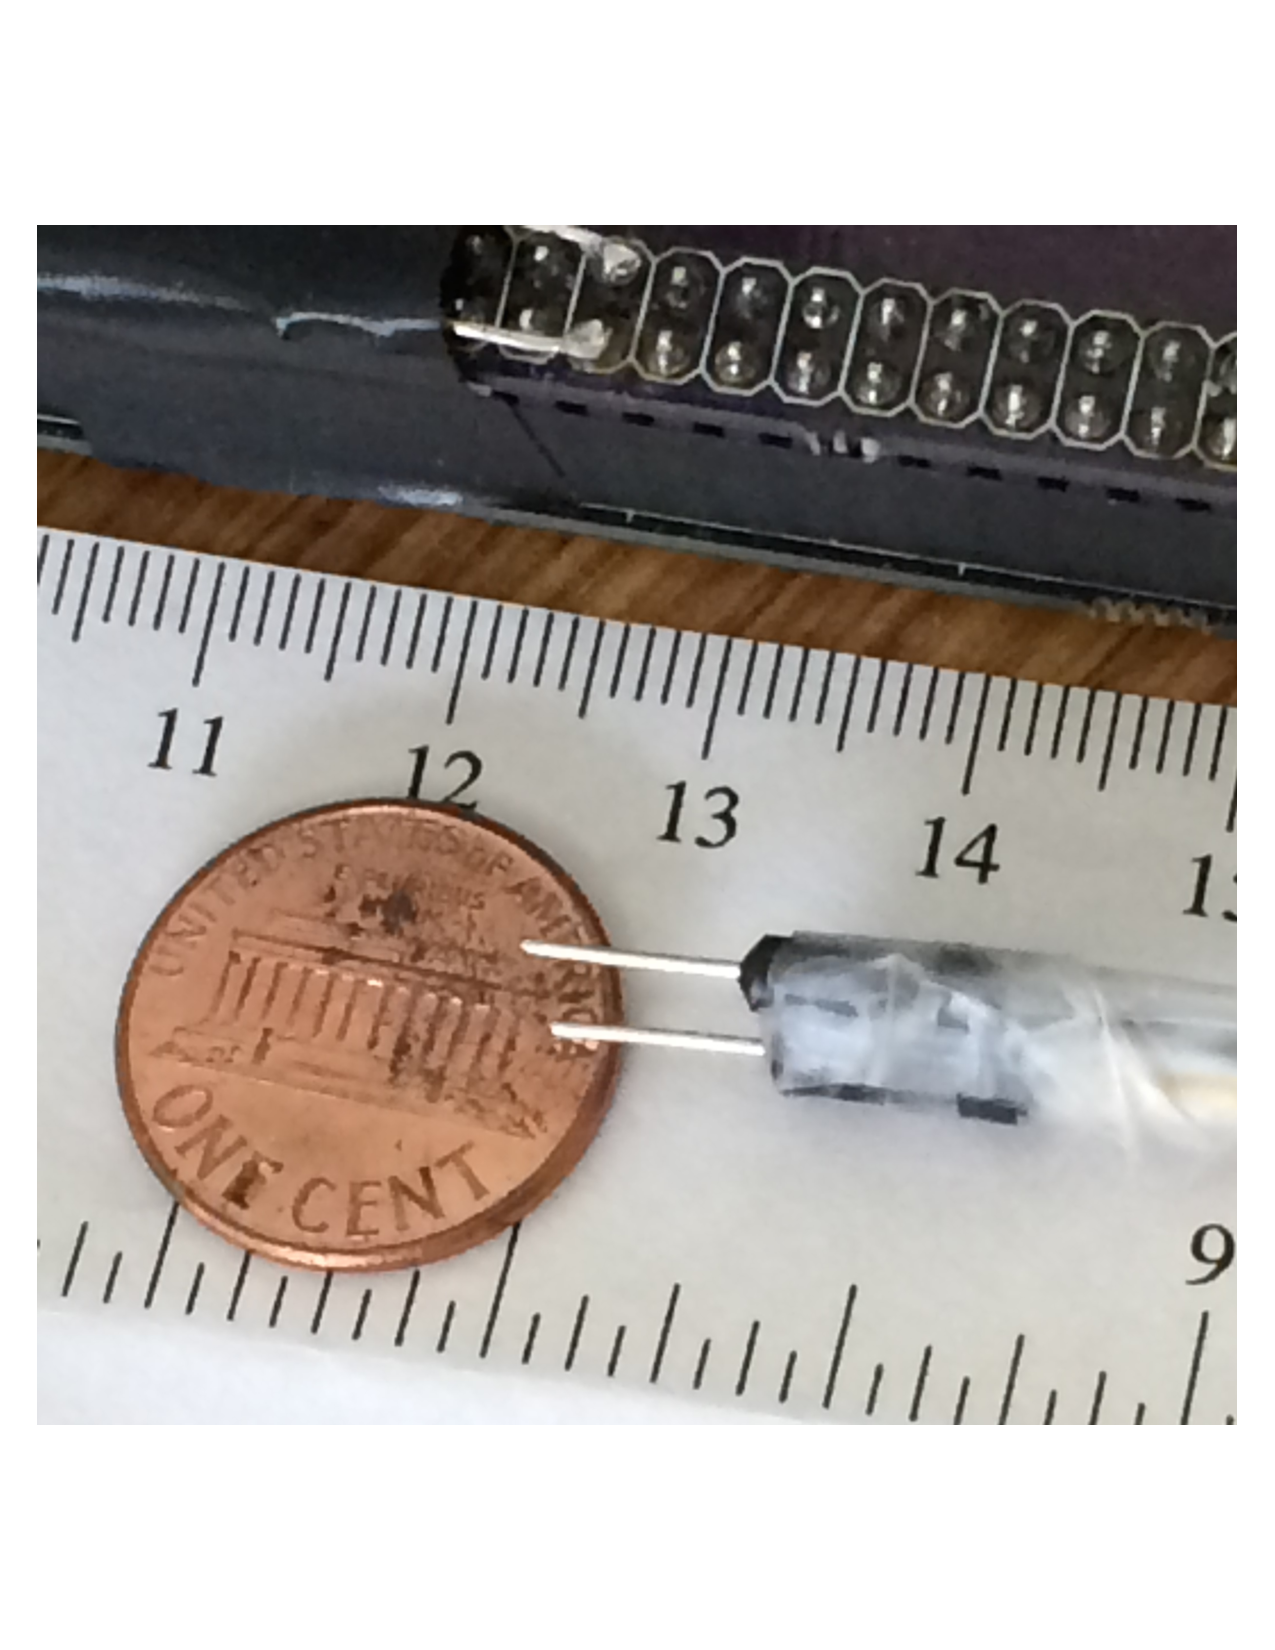
\includegraphics[width=0.3 \linewidth]{electrode}
\caption{Electrodes - made out of two tin-coated male copper pins typically used as jumper cables for breadboard design.}
\end{center}
\end{figure}

\section{Results}
\subsection{Optical density-based quantification}
\begin{knitrout}
\definecolor{shadecolor}{rgb}{0.969, 0.969, 0.969}\color{fgcolor}\begin{figure}[]


{\centering 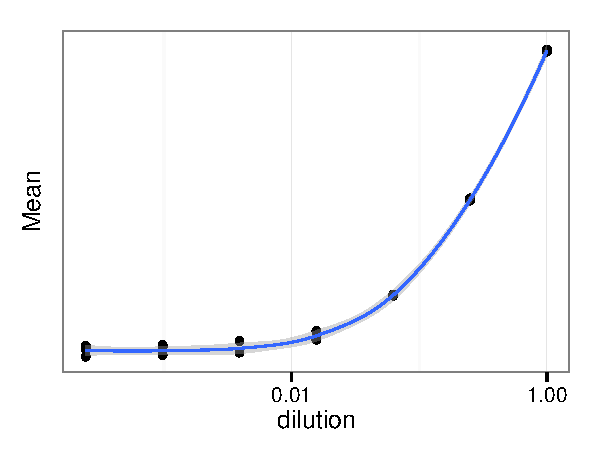
\includegraphics[width=\maxwidth]{figure/odplot} 

}

\caption[Optical density at 600 nm as a function of dilution]{Optical density at 600 nm as a function of dilution\label{fig:odplot}}
\end{figure}


\end{knitrout}


\subsection{Typical impedance curves} 
\begin{knitrout}
\definecolor{shadecolor}{rgb}{0.969, 0.969, 0.969}\color{fgcolor}\begin{figure}[]


{\centering 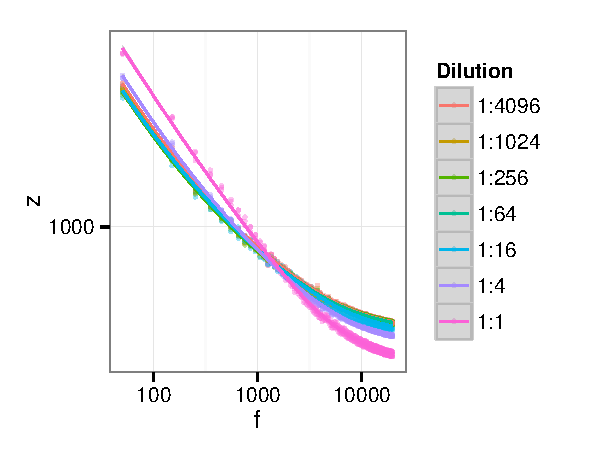
\includegraphics[width=\maxwidth]{figure/impedance_curves} 

}

\caption[Frequency response as a function of dilution]{Frequency response as a function of dilution\label{fig:impedance_curves}}
\end{figure}


\end{knitrout}


\subsection{Linear and nonlinear models}
We want to simplify the impedance curve to a few parameters, and see if these parameters are predictive of the optical density. 
We first test a simple model where we fit a straight line to the frequency response in the log-log space. 
$$
\mathrm{log}(z) = \mathrm{Slope} \times \mathrm{log}(f) + \mathrm{Intercept}
$$
where $z$ is impedance in ohms and $f$ is frequency in Hz. Since this is a linear model, \emph{Slope} and \emph{Intercept} are correlated. We can test if the slope is predictive of the quantity \emph{Mean}, which signifies optical density. Note that we weigh the regression for the higher frequencies to fit the higher frequency spectrum better. The results are not too different without this weighted regression however. 

\begin{knitrout}
\definecolor{shadecolor}{rgb}{0.969, 0.969, 0.969}\color{fgcolor}\begin{kframe}
\begin{verbatim}
## 
## Call:
## lm(formula = Mean ~ Slope, data = growth_data)
## 
## Residuals:
##      Min       1Q   Median       3Q      Max 
## -0.10095 -0.02387  0.00419  0.03542  0.05816 
## 
## Coefficients:
##             Estimate Std. Error t value Pr(>|t|)    
## (Intercept)   -1.345      0.058   -23.2   <2e-16 ***
## Slope         -5.894      0.216   -27.2   <2e-16 ***
## ---
## Signif. codes:  0 '***' 0.001 '**' 0.01 '*' 0.05 '.' 0.1 ' ' 1
## 
## Residual standard error: 0.0441 on 34 degrees of freedom
## Multiple R-squared:  0.956,	Adjusted R-squared:  0.955 
## F-statistic:  743 on 1 and 34 DF,  p-value: <2e-16
\end{verbatim}
\end{kframe}
\end{knitrout}


As seen above, a near perfect correlation exists between the slope of the frequency response and the optical density. 

Given the interesting curvilinear profile of the impedance curve, we are interested in seeing if we can fit a slightly more mechanistic model to the curve. We assume that the media between the electrodes can be modeled as a pure resistor in series with a Warburg-like element. Typically a Warburg element is considered an appropriate choice when measuring impedance of a diffusion-limited process, as is the case here. The typical complex Warburg impedance is given by:

$$
Z_W = \frac{A_W}{\sqrt{\omega}} (1 - i)
$$
where $Z_W$ is the complex Warburg impedance, $A_W$ is a scaling factor and $\omega$ is the angular frequency. The exponent of 0.5 of $\omega$ comes from an assumption of planar electrode geometry, which is not the case in our system. In any case, we modify the Warburg term slightly by allowing the exponent to vary freely from 0.5. We used the following formulation:

$$
Z_W = \frac{A_W}{\omega^\eta} (1 - i)
$$

where $A_W$ and $\eta$ were solved from $f$ and $z$ data. 

An example of the degree to which such a model fits the data is shown below:

\begin{knitrout}
\definecolor{shadecolor}{rgb}{0.969, 0.969, 0.969}\color{fgcolor}\begin{figure}[]


{\centering 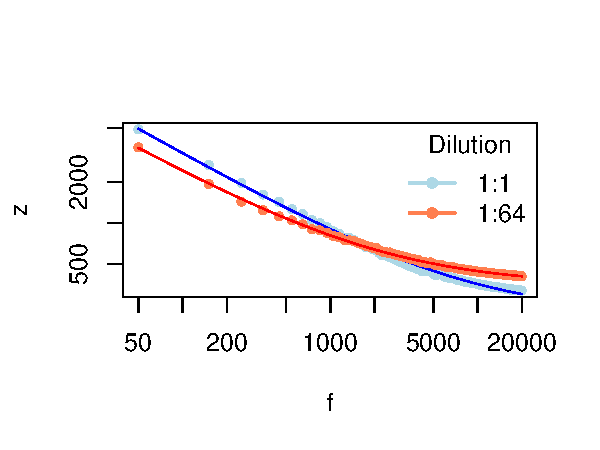
\includegraphics[width=\maxwidth]{figure/nlsmod_fit} 

}

\caption[Warburg-like impedance model fit to data]{Warburg-like impedance model fit to data\label{fig:nlsmod_fit}}
\end{figure}


\end{knitrout}


A reasonably good fit, though the fit may be improved for lower dilutions. Taken together, the three terms adequately capture the observed optical density as can be seen from the regression below. 

\begin{knitrout}
\definecolor{shadecolor}{rgb}{0.969, 0.969, 0.969}\color{fgcolor}\begin{kframe}
\begin{verbatim}
## 
## Call:
## lm(formula = Mean ~ Warburg + Resistance + Exponent, data = growth_data)
## 
## Residuals:
##      Min       1Q   Median       3Q      Max 
## -0.09174 -0.02161  0.00424  0.03195  0.06101 
## 
## Coefficients:
##              Estimate Std. Error t value Pr(>|t|)    
## (Intercept)  3.47e+00   5.01e-01    6.93  7.5e-08 ***
## Warburg      8.67e-06   7.79e-07   11.13  1.6e-12 ***
## Resistance  -2.64e-03   2.20e-04  -12.00  2.2e-13 ***
## Exponent    -5.04e+00   8.86e-01   -5.69  2.6e-06 ***
## ---
## Signif. codes:  0 '***' 0.001 '**' 0.01 '*' 0.05 '.' 0.1 ' ' 1
## 
## Residual standard error: 0.0439 on 32 degrees of freedom
## Multiple R-squared:  0.959,	Adjusted R-squared:  0.955 
## F-statistic:  250 on 3 and 32 DF,  p-value: <2e-16
\end{verbatim}
\end{kframe}
\end{knitrout}



\end{document}
